\documentclass{emonides-cv}

\setsansfont{Dotum}

\begin{document}
  
\rhead {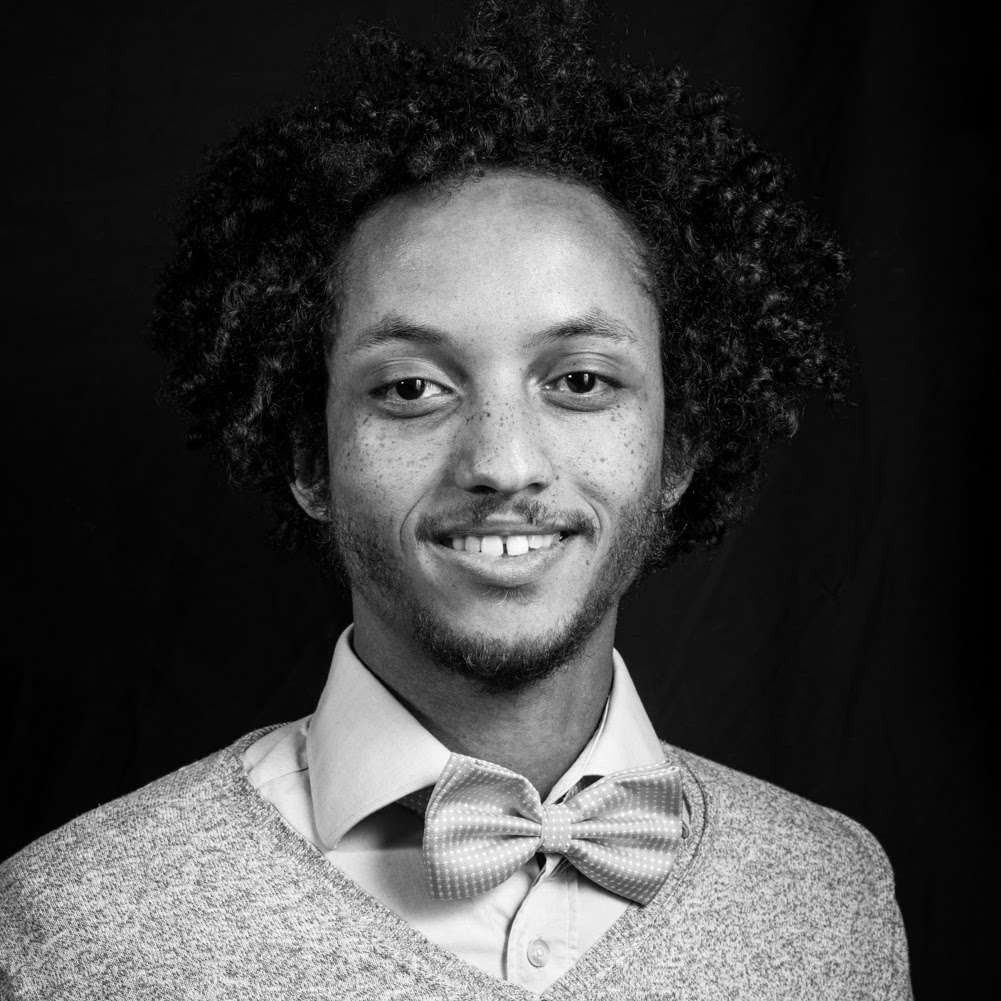
\includegraphics[width=1.5cm]{photoCV.jpg}}
  {Emonides} {Pierre-Emmanuel}
  {Software/Backend Engineer}
  { Overtoom 555B\\
    1054LK Amsterdam\\
    Netherlands\\
    +33 665 44 88 14\\
    pemonides@gmail.com\\
    }

I'm a full stack software engineer, I have 6+ years experience with backend and mobile development.
I would like to keep working on Backend/Software development, with languages like C\#, Python or Go.
\section{Experience}
\begin{entrylist}
  \entry
    {Since 2018}
    {Python Backend, \href{https://www.sanoma.nl/over-sanoma-nl/}{Sanoma} {\normalfont Amsterdam}}
    {2 years Full Time}
    {As \emph{\textbf{Python3 Developer}. I joined the team in charge of developing all common core services used by Sanoma magazines. First for Sanoma Account Solution, the cross-magazine user database. Then worked on the Dynamic Image Service Provider used by all media owned by Sanoma. Traffic:2M Image Requested/24h. For a total of ~150M Images Stored.
    I used technologies as \textbf{AWS, Terraform, ELK, Python3.6, FastAPI, Pillow, PostgreSQL, MongoDb}.}}
  \entry
    {2016-2018}
    {CTO at \href{https://fr.linkedin.com/company/360boost/}{360Boost}  {\normalfont Paris}}
    {2 years Full Time}
    {\emph{Technical-lead, conception, planning, development and deployment of \textbf{C\# Android/IOS app, NodeJs} Servers.
     Management of clusters on \textbf{Gcloud, Kubernetes, Ansible}. Team-lead with 4 employees (1500 Users, B2B + B2C).
    \\360Boost is a native IOS/Android app, built with Xamarin.Forms, I did the conception, development on this app.
    Then I had to lead 2 Interns and 1 employee in the next steps of development.
    360Boost is also a B2B solution with a \textbf{React} WebApplication, I managed one React Developer
    in the development and deployment.
    The backend is a NodeJS Rest Server developed with Express. I did all the development steps, from conception
    to Cluster deployment on Google Cloud using Kubernetes and Ansible}}
  \entry
    {2015}
    {Mobile Consultant, \href{https://www.docapost.com/en/}{Docaposte} {\normalfont Paris}}
    {6 months Full Time}
    {\emph{\textbf{Android/Java Developer}. Sent to a major client of Acensi Docapost, I worked on a solution for Digitizing contracts.
    During this experience I used technologies as \textbf{Digital Signatures, SSL}.
    I had to develop on Java/Tomcat servers, as well as mobile applications on \textbf{Java Android}.}}
  \entry
    {2014-2015}
    {Consultant, \href{https://www.acensi.fr/}{Acensi} {\normalfont Paris, La Défense}}
    {1.5 years Full time}
    {\emph{\textbf{C\# WPF .Net4.5} development for a Finance Banking software, \href{https://www.eurocaution.net/}{Eurocaution}.
    I became team-lead for this project (15 developers, 3 teams). Two-week Sprints, daily stand-up meetings, sprint retrospective etc...
    \\Then \textbf{C\# Xamarin} Mobile development on a para-medical application called \href{http://www.triacys.com/}{Triacys}.
    I worked on a custom Android Kernel for BeagleBoard, then Android Tablets. I also developped custom userspace-drivers for devices like blood pressure monitor
    (2 developers). Agile management method with client review meetings. }}
  \entry
    {2012}
    {C++ developer, \href{https://www.acensi.fr/}{Sogeti High Tech} {\normalfont Rennes, France}}
    {6 months}
    {\emph{\textbf{C++/QT} Developer for a user interface testing solution called\href{https://www.eurocaution.net/}{Takt Engine}.
    I extended the capabilities of the testing solution. I worked with \textbf{OpenCV} to detect bad artefacts during tests }}
  \entry
    {2010}
    {Lua GameDeveloper, \href{https://www.giantbomb.com/white-birds-productions/3010-5637/}{White Birds} {\normalfont Paris, La Défense}}
    {6 months}
    {\emph{Lua Developer for Point-and-click games, \href{https://www.bigfishgames.com/games/6859/cardboard-castle/}{Cardboard Castle}. \href{https://www.wikiwand.com/fr/White_Birds_Productions}{Last King of Africa}}}
\end{entrylist}

\vspace{1.5cm}

\section{Side Projects}
\begin{entrylist}
  \entry
    {2018}
    {Cryptocurrency exchanges arbitrage bot {\normalfont }}
    {Personal projet}
    {\emph{Part of the \textbf{Python} development team. Retrieve the orderbook/tick data of different exchanges through websockets for analytics. }}
  \entry
    {2017-2018}
    {Rentfirst.nl {\normalfont  (Co-Founder)}}
    {Startup}
    {\emph{Rental housing aggregator for the Amsterdam area. \\
    I was the main developer of a \textbf{NodeJS REST API} back-end.
    I also succesfully inplemented an IOS/Android application listing the offers}}
  \entry
    {2016-2017}
    {\href{http://www.teamgeny.com/}{Team-Geny} {\normalfont Mobile Developer}}
    {Startup}
    {\emph{Creating Mobile applications using Xamarin/JavaAndroid}}
  \entry
    {Since 2014}
    {\href{https://play.google.com/store/apps/developer?id=EpicBacon}{EpicBacon} {\normalfont Main-Developer}}
    {Personal projet}
    {\emph{Main developper of EpicBacon. During my freetime I develop mobile applications and web solutions using \textbf{Unity3D} and \textbf{Java/AndroidSDK}.
    I also do 3Dmodeling with 3DsMax for 3Dprinting  }}
\end{entrylist}
\section{Skills}
\normalsize
\textbf {Daily Usage:}   C\#, JavaScript/NodeJS, Python\\
\normalsize {  Mobile Development, Xamarin.Forms/Android, WPF, AWS, Google Cloud}\\
\textbf {Occasionally:} Java, Go, C, C++ \\
Unity3D, Azure\\
\textbf {Deployment:} Terraform, Ansible, Kubernetes, Docker, Git Workflow\\
\textbf {Databases:} MongoDb, ElasticSearch, PostgreSQL, MySql\\
\textbf {Systems:} Nginx, (Arch)Linux/*Bsd \\
\textbf {Misc:} Jira, Mantis, \LaTeX, Gimp, Photoshop, 3DSMax\\
\textbf { Certifications: } 70-483 Programming in C\#\\
\textbf { Languages: } French native, English fluent

\section{Education}
\begin{entrylist}
  \entrytwo
    {2013-2014}
    {Master's degree {\normalfont Computer science }}
    {Epitech European Institute of Information Technology, Paris} {Project-oriented pedagogy : around 40 projects achieved alone or within a team.}
  \entrytwo
    {2012-2013}
    {Student exchange program  {\normalfont  Mobile\&Game development }}
    { {\sffamily 계명대학교} Keimyung University, Daegu South Korea} {}
  \entrytwo
    {2009–2012}
    {Bachelor  {\normalfont Computer Science Programming and software design}}
    {Epitech, Rennes} {}
  \entry
    {2006–2009}
    {French Baccalauréat ES. {\normalfont with honors. }}
    {Lycée Schœlcher, Fort-de-France} { Specialization in mathematics }
\end{entrylist}
\sectiontwo{Activities}
\normalsize Kickboxing, Salsa, 3D Modeling, Drawing, Ski, MotorBike
\end{document}
